
\section{Two-Sample Tests}

\par If we split a quantitative variable into two groups based on a binary variable, we can test whether the two samples have equal medians and/or variance. Box plots were generated for each of the possible variable choices to identify potential differences. The author selected three pairings of variables whose boxplots  seemed to show significantly different medians, shown in Figure \ref{fig:twosample_boxplots} along with histograms to give the reader a sense of the distribution's shape. We see that each distribution is somewhat right-skewed, and the white age distribution seems skinnier than the non-white distribution in the first histogram.

\begin{figure}[h]
    \centering
    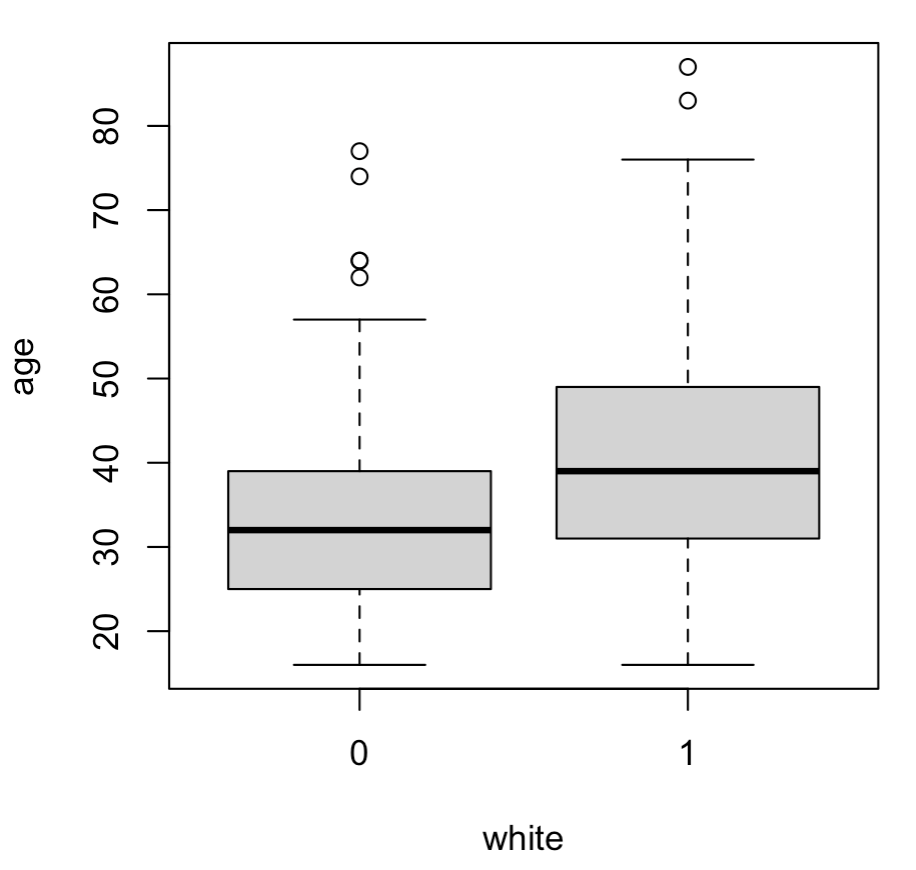
\includegraphics[scale=.3]{boxplot_age_white.png}
    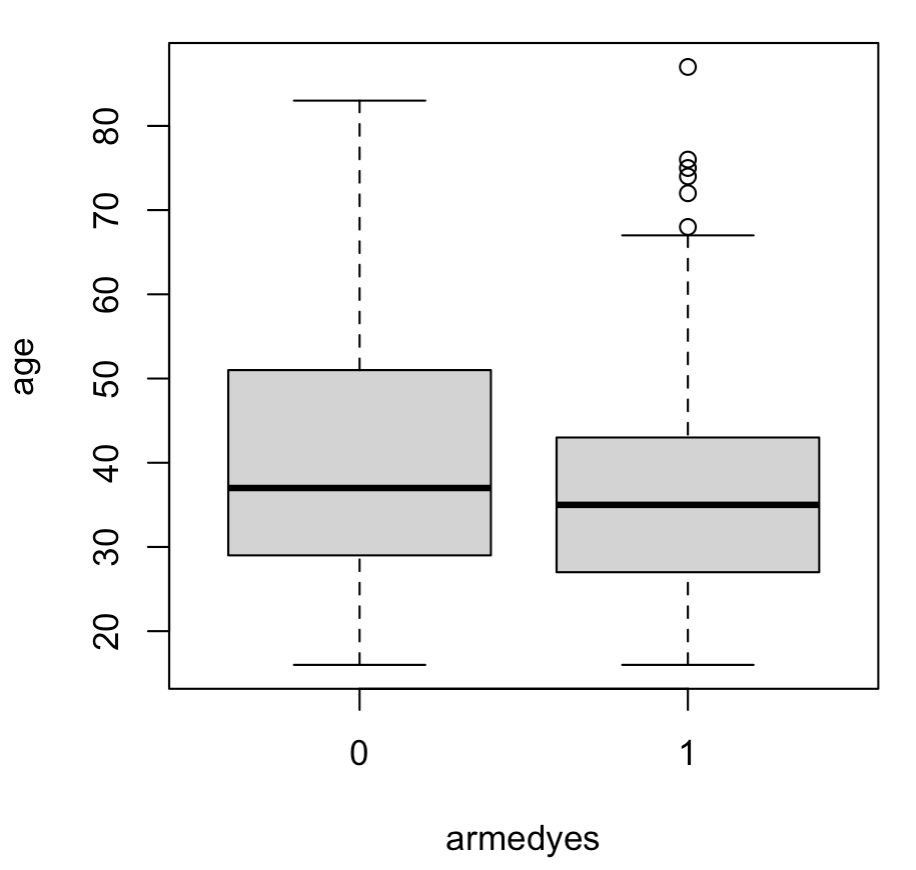
\includegraphics[scale=.3]{boxplot_age_armedyes.png}
    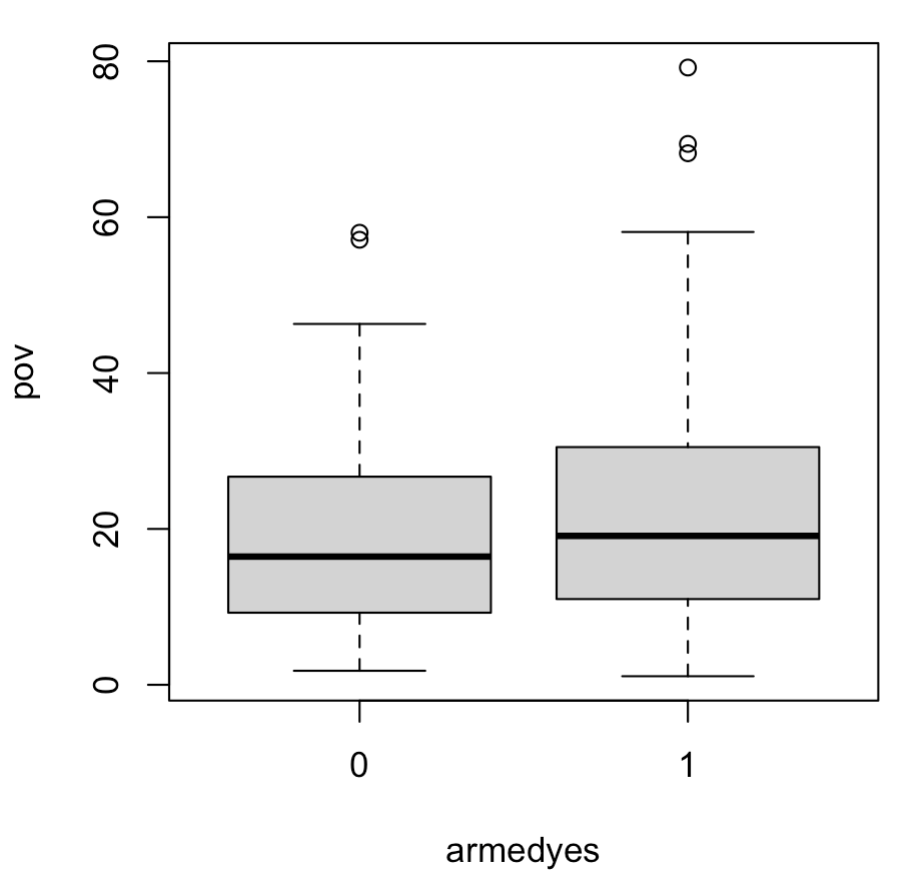
\includegraphics[scale=.3]{boxplot_pov_armedyes.png}
    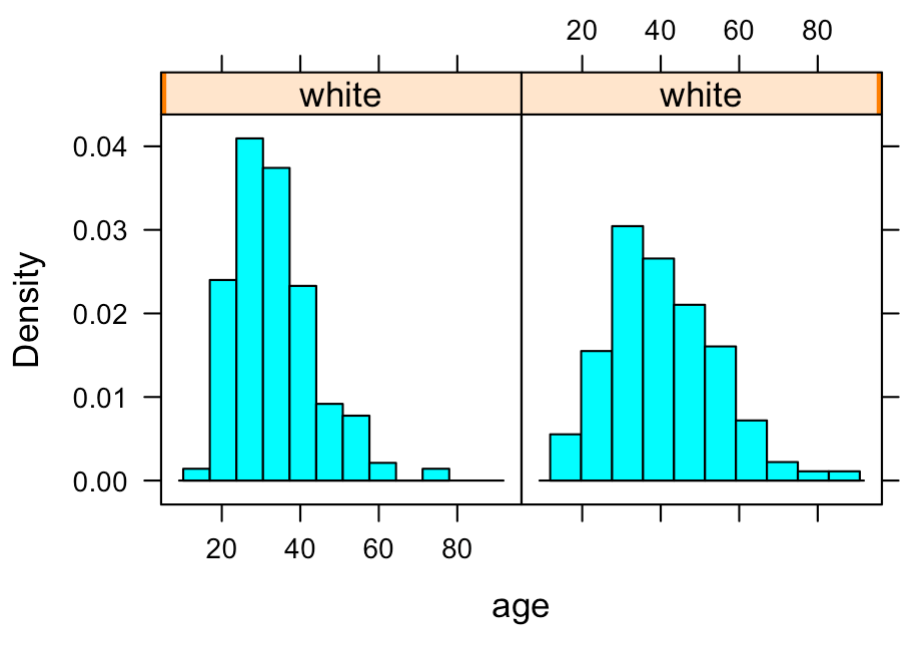
\includegraphics[scale=.3]{histplot_age_white.png}
    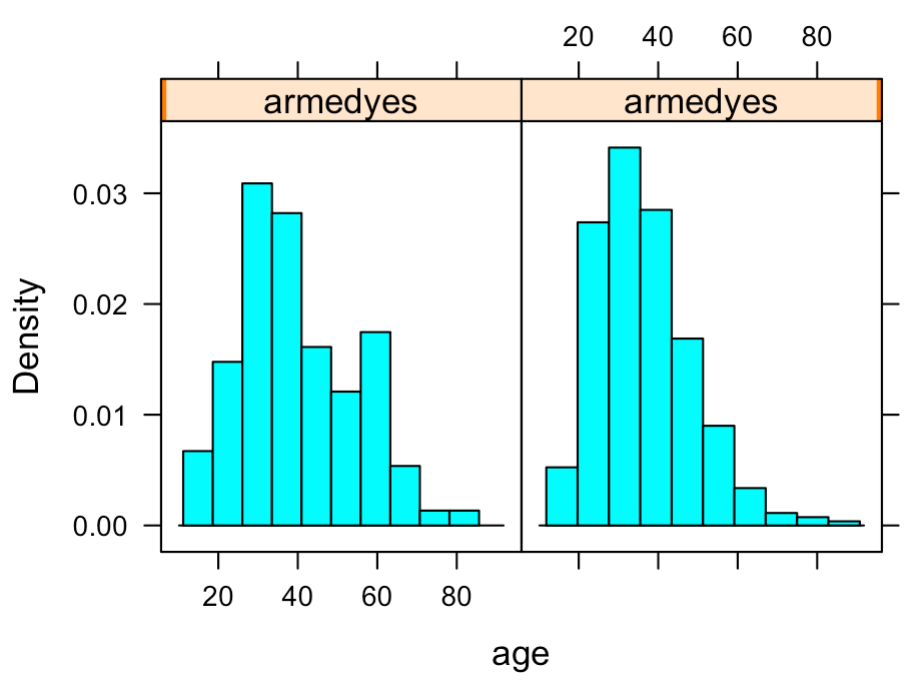
\includegraphics[scale=.3]{histplot_age_armedyes.png}
    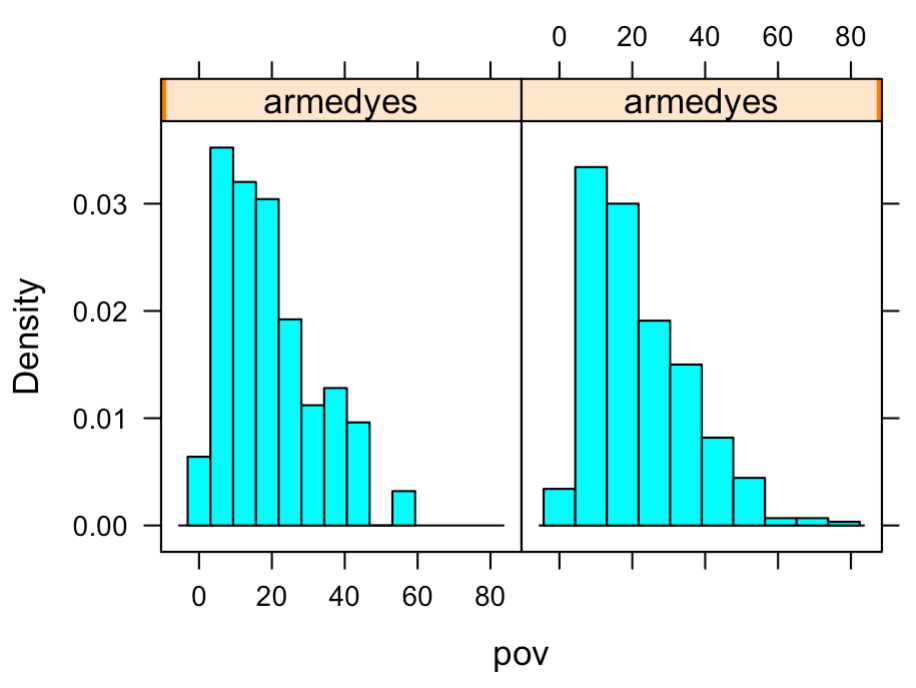
\includegraphics[scale=.3]{histplot_pov_armedyes.png}
    \caption{Box plots and histograms of three quantitative-binary variable pairs }
    \label{fig:twosample_boxplots}
\end{figure}

\subsection{Age vs. Whiteness: Parametric Analysis}

\par Our data includes 229 white victims and 209 nonwhite victims. In order to find a significant difference between the average age of these two populations, our first instinct might be to conduct a $t$-test. Let $\mu_W$ be the mean age of white victims and $\mu_N$ be the mean of nonwhite victims. Our null hypothesis is that these two means are equal, or equivalently, their difference $\mu_W - \mu_N = 0$. Our estimate of the difference is simply the difference in the mean ages of our two samples, which turns out to be 7.259 years.

\par \bigskip But is this difference significant? Using the base R function \texttt{t.test()}, we obtain a $p$-value of $1.038*10^{-9}$ and a 95 percent confidence interval of $(4.973, 9.544)$. If this test were valid, we would reject the null hypothesis and declare with 95 percent confidence that white victims are between 4.973 and 9.544 years older than nonwhite victims on average.

\par \bigskip Unfortunately, a quick look at some diagnostic plots shows us that the conditions for inference based on the $t$-test are not met. Figure \ref{fig:ttest1_plots} shows a plot of the residuals vs. fitted values from our model,\footnote{To create the plots in Figures \ref{fig:ttest1_plots} and \ref{fig:ttest2_plots}, the author used one-way ANOVA tests, which in the two-sample case are equivalent to $t$-tests.} as well as a normal probability plot of the residuals. The residuals for the nonwhite population seem to be less widely distributed than for the white population, calling the equal variance assumption into question. We can further test for unequal variance with Levene's test. Using the R function \texttt{levene.test()} from the package \texttt{lawstat}, we obtain a $p$-value of .000413 and conclude that the variances of the two populations are indeed unequal.

\vspace{.2in}

\begin{figure}[h]
    \centering
    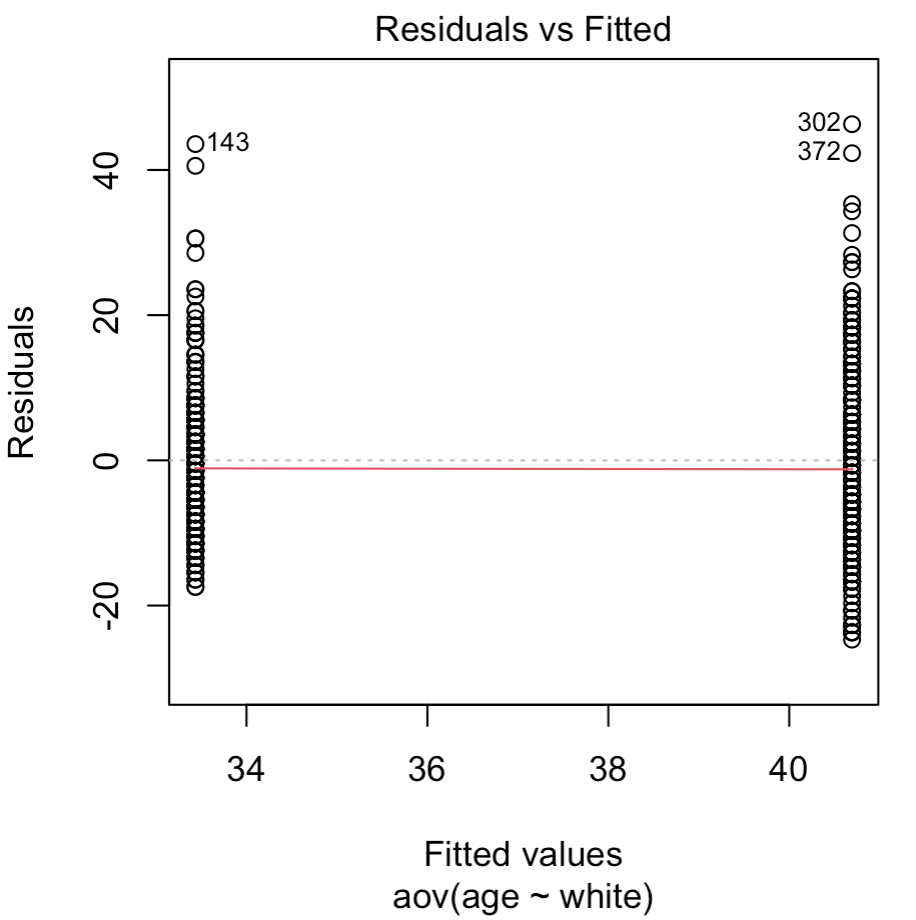
\includegraphics[scale=.4]{ttest1_plot1.png}
    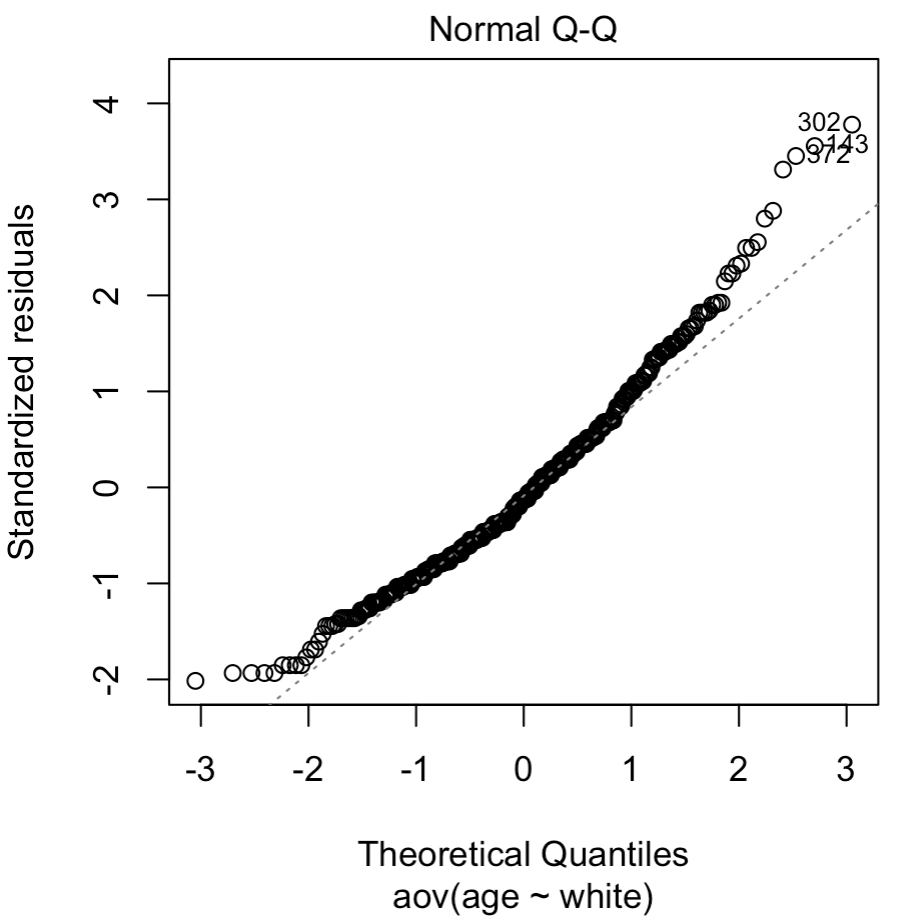
\includegraphics[scale=.4]{ttest1_plot2.png}
    \caption{Diagnostic plots for the two-sample $t$-test of $age$ vs. $white$}
    \label{fig:ttest1_plots}
\end{figure}

\par \bigskip Furthermore, we have evidence that our populations are not distributed normally. The normal probability plot shows residuals that depart strongly from the expected normal curve at both tails. We can also conduct the Anderson-Darling test for normality. Using the R function \texttt{ad.test()} from the package \texttt{nortest}, we obtain a $p$-value of $1.013*10^{-7}$ and conclude that our residuals do not follow the normal distribution. Clearly, any inference we make from the standard $t$-test on these two samples would be invalid.

\newpage

\par \bigskip Perhaps a transformation on $age$ will satisfy the conditions for the $t$-test. In Figure \ref{fig:ttest1_plots} we see upper outliers in the boxplots and a right skew in the histograms. The square root of age might have a more symmetric distribution. Sure enough, our plots of $\sqrt{age}$ vs. $white$ and the new $t$-test residuals (shown in Figure \ref{fig:ttest1_transformed_plots}) depict a distribution that looks much closer to the normal curve. However, Levene's test of the transformed variance returns a $p$-value of 0.00844, and the Anderson-Darling test returns a $p$-value of 0.0396. We still reject their null hypotheses of equally-varying and normal residuals.

\begin{figure}[h]
    \centering
    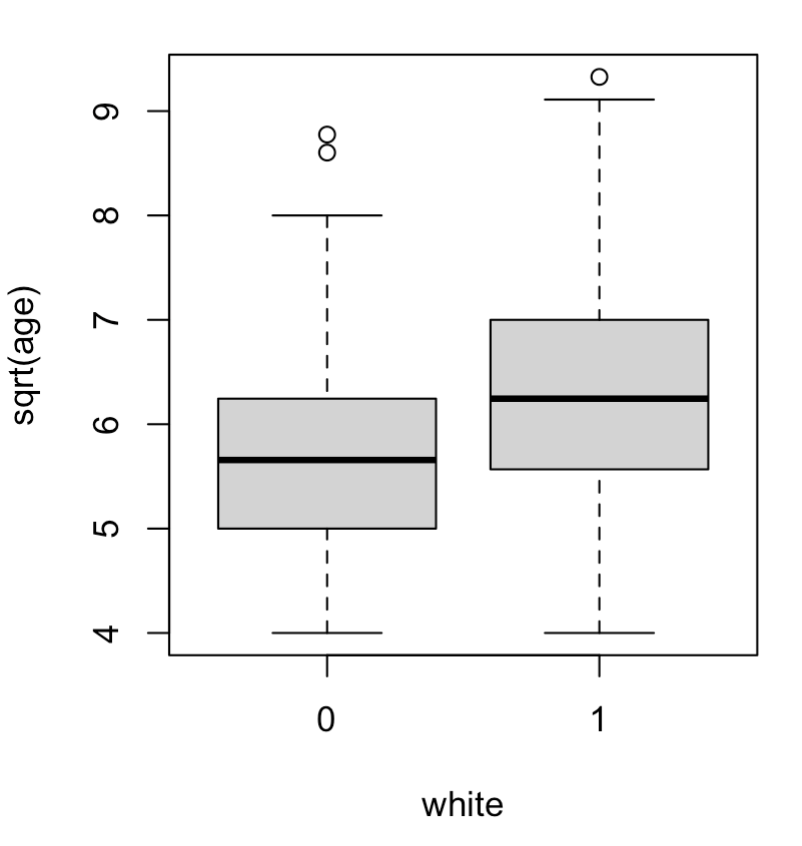
\includegraphics[scale=.4]{boxplot_sqrtage_white.png}
    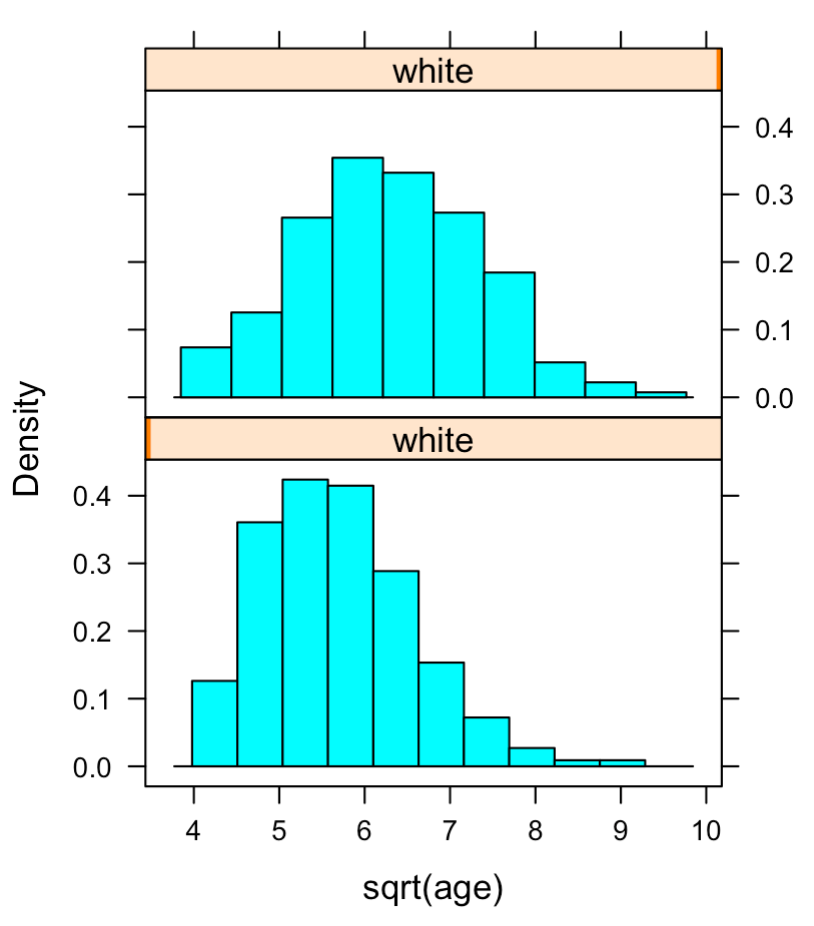
\includegraphics[scale=.4]{histplot_sqrtage_white.png}
    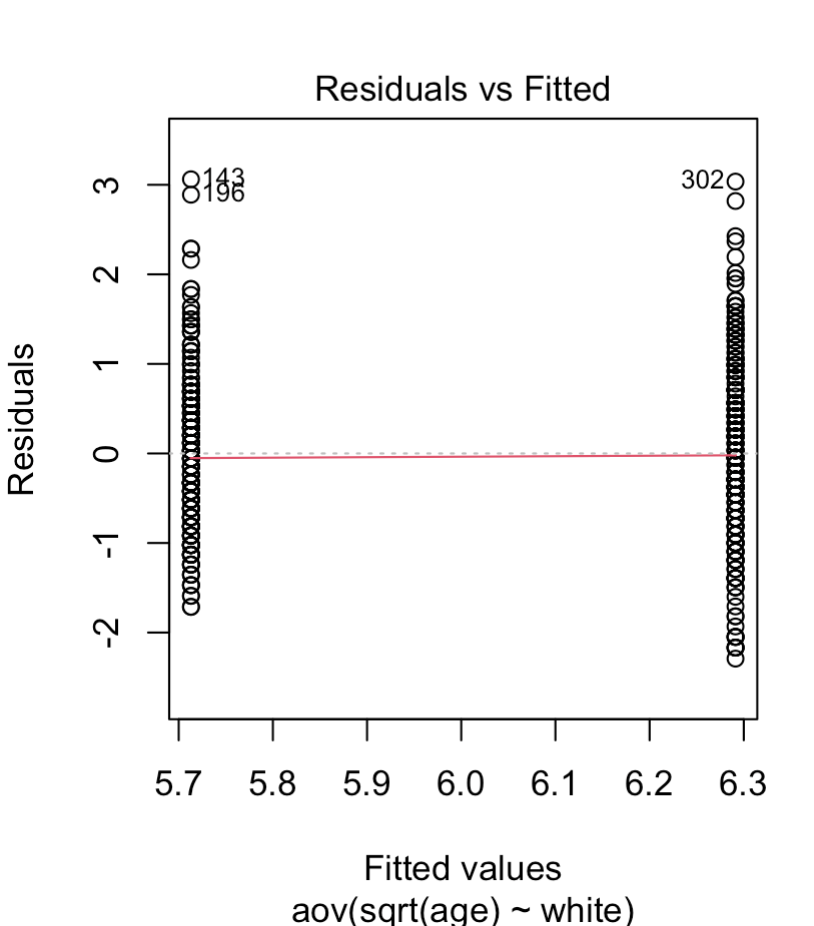
\includegraphics[scale=.4]{ttest1_transformed_plot1.png}
    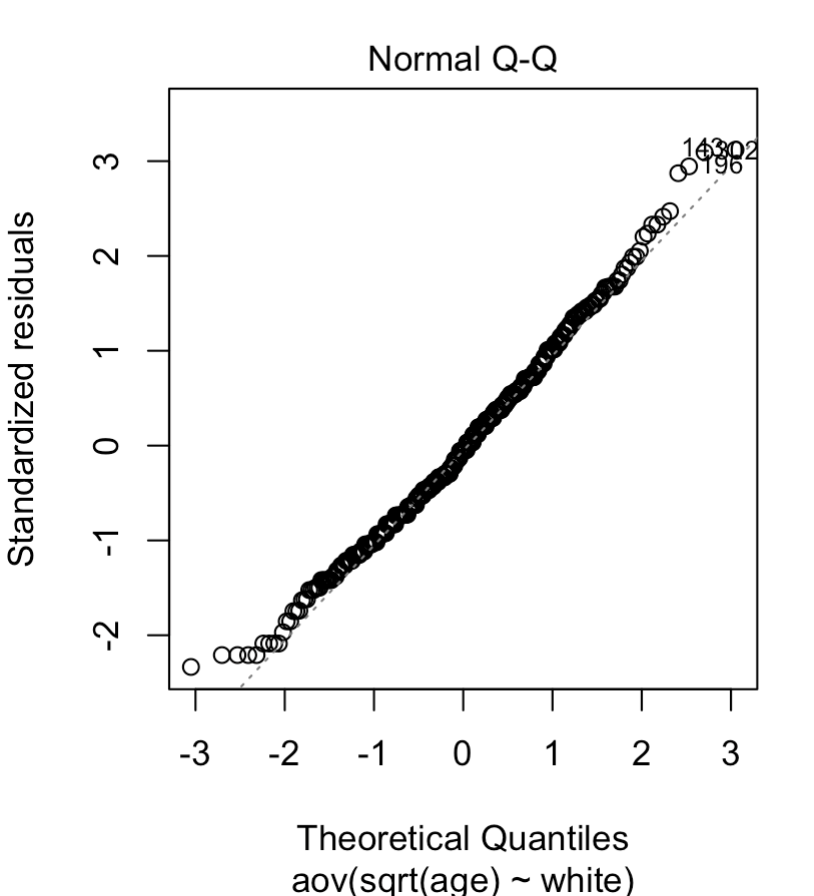
\includegraphics[scale=.4]{ttest1_transformed_plot2.png}
    \caption{Plots of $\sqrt{age}$ vs. $white$}
    \label{fig:ttest1_transformed_plots}
\end{figure}

\par For the sake of comparison with our nonparametric procedures, we convert the estimates from the $t$-test on $\sqrt{age}$ against $white$ back into regular years and report them. Though their distribution is still invalid for the $t$-test, it is an improvement on the untransformed model and its conclusions are slightly more representative of the truth. Our new $p$-value is $1.381*10^{-9}$. Our new estimate is the difference between the squared estimates of mean $\sqrt{age}$, which comes out to 6.941. We form the new confidence interval by taking the squared mean $\sqrt{age}$ of white victims and subtracting the squared difference between the mean $\sqrt{age}$ of white victims and the lower bound of our confidence interval, then doing the same with the upper bound. This new interval is $(4.810, 9.004)$.

\par \bigskip In light of the problematic distribution of age against whiteness, we turn to nonparametric methods for a more robust analysis of the two variables.

\subsection{Age vs. Whiteness: Nonparametric Analysis}

\par \bigskip We will first determine whether the distributions underlying our two populations are dispersed equally. Setting $\gamma^2 = \frac{var({\sqrt{age}}_{white})}{var({\sqrt{age}}_{nonwhite})}$, we seek to determine whether the ratio of the two population variances $\gamma^2$ is significantly far from 1 in either direction.

\par \bigskip Our result from Levene's test suggests that these variances are unequal. However, we see from Figure \ref{fig:ttest1_plots} that the data contains several outliers, to which Levene's test is very sensitive. In comparison, the Miller jackknife procedure is much more resilient to outliers because its test statistic is adjusted based on the contribution of each observation to the overall mean. We can make a more robust conclusion about the variances of these two populations by applying the jackknife procedure.

\bigskip \textbf{Miller jackknife test}

\bigskip $H_0: \gamma^2 = 1$

$H_3: \gamma^2 \not= 1$ \hspace{1in} Reject $H_0$ if $|Q| \ge z_{\alpha/2}$.

\par \bigskip Using the custom R function \texttt{jackKnife()}, we find that $Q = 2.420$ and obtain a $p$-value of 0.00777, which is quite similar to that of Levene's test. We also obtain an estimate for the ratio between the variances of the populations, $\bar{\gamma}^2 = 1.581$, and the associated 95 percent confidence interval $(1.141, 2.191)$. In other words, we are 95 percent confident that the variance in age for white victims is between 1.141 and 2.191 times larger than that of nonwhite victims.

\par \bigskip Now we move on to determining whether the median ages are different for our two populations. In light of our rejection of the null hypothesis with the Miller jackknife, we should conduct the Fligner-Policello test, which does not assume equality of variance. We need not transform and untransform $age$ for this test: it is based on the ranks of observations relative to each other, and since the square root is an increasing function, it does not change the rankings of observations at all. Therefore, the test will not conclude anything differently before and after transformation. Additionally, since our sample has many observations and because it reduces computing time greatly, we will use the large-sample approximation (LSA) of the Fligner-Policello test.

\bigskip \textbf{Fligner-Policello test}

\bigskip $H_0: \theta_{white} = \theta_{nonwhite}$

$H_3: \theta_{white} \not= \theta_{nonwhite}$ \hspace{1in} Reject $H_0$ if $|\hat{U}| \ge z_{\alpha/2}$.

\par \bigskip Using the R function \texttt{pFligPoli()} from the package \texttt{NSM3}, we find that $\hat{U} = 6.353$ and obtain a $p$-value of $2.112*10^{-10}$. Thus we reject the null hypothesis and conclude that the median age of white victims is different than that of non-white victims.

\par \bigskip For an estimate of the true difference in median $\theta_{white} - \theta_{nonwhite}$, we can use the Hodges-Lehmann $\hat{\Delta}$, which is the median of the differences between each measurement of $age_{nonwhite}$ and $age_{white}$. Using the base R function \texttt{wilcox.test()}, we see that $\hat{\Delta} = 7.000$. In other words, we estimate that white victims are roughly 7 years younger than nonwhite victims on average. The output also finds a confidence interval of $(5.000, 9.000)$, but that is meaningless if the variances of our populations are unequal.

\par \bigskip Table \ref{tab:twosample1_results} summarizes the results obtained from our tests of age broken down by whiteness. It appears that the true difference in means (and our sample size) is large enough to make the conclusions of these tests very similar. 

\vspace{.2in}

\begin{table}[h]
    \centering
    \begin{tabular}{|l|c|c|c|c|}
        \hline
        \textbf{parameter} & \textbf{procedure} & \textbf{p-value} & \textbf{estimate} & \textbf{95 pct. CI}\\
        \hline
        Location & $t$-test & $1.381*10^{-9}$ & $\hat{\mu}_W-\hat{\mu}_N = 6.941$ & $(4.810, 9.004)$\\
        & Fligner-Policello & $2.111*10^{-10}$ & $\hat{\Delta} = 7.000$ & not meaningful\\
        \hline
        Dispersion & Levene's test & 0.00844 & -- & --\\
        & Miller jackknife & 0.00777 & $\bar{\gamma}^2 = 1.396$ & $(1.065, 1.829)$\\
        \hline
    \end{tabular}
    \caption{Results for $age$ vs. $white$}
    \label{tab:twosample1_results}
\end{table}

\subsection{More Two-Sample Analysis}

\par For the remainder of the paper, we will continue applying a square root to $age$ and all other quantitative variables, as it improves conditions in every case.

\par \bigskip Our second analysis, of age broken down by whether or not the victim was armed, goes quite similarly to our first. There are 338 armed and 100 unarmed victims in the dataset. This time, the Anderson-Darling test still rejects the normality condition, but Levene's test returns a $p$-value of 0.0850, hovering right on the brink of the common significance level of $\alpha = 0.05$. The Miller jackknife returns a similar $p$-value of 0.0584. Therefore, in addition to the Fligner-Policello test, we proceed with the Wilcoxon rank sum test using \texttt{wilcox.test()} and obtain a meaningful 95 percent confidence interval for the difference in population medians $\theta_{A}-\theta_{U}$. Though both nonparametric tests for unequal means are less certain than the $t$-test, they still reject the null at alpha levels .05 and higher. Full results are shown in Table \ref{tab:twosample2_results}.

\begin{table}[h]
    \centering
    \begin{tabular}{|l|c|c|c|c|}
        \hline
        \textbf{parameter} & \textbf{procedure} & \textbf{p-value} & \textbf{estimate} & \textbf{95 pct. CI}\\
        \hline
        Location & $t$-test & 0.0328 & $\hat{\mu}_U-\hat{\mu}_A = -3.274$ & $(-6.403, -0.266)$\\
        & rank sum & 0.0400 & $\hat{\Delta} = -3.000$ & $(-6.000, -0.0000587)$\\
        & Fligner-Policello & 0.0454 & -- & --\\
        \hline
        Dispersion & Levene's test & 0.0850 & -- & --\\
        & Miller jackknife & 0.0584 & $\bar{\gamma}^2 = 0.709$ & (0.574, 1.010)\\
        \hline
    \end{tabular}
    \caption{Results for $age$ vs. $armedyes$}
    \label{tab:twosample2_results}
\end{table}

\par As for $pov$ vs. $armedyes$, normal residuals are again soundly rejected, but neither variance test could conclude that the populations have different scales. We proceed only with the Wilcoxon rank sum test, which fails to find a difference in medians. Therefore, we do not have sufficient evidence to conclude that the populations are distributed differently in any way. In this case, we see that the rank sum test is slightly less confident than the $t$-test, while the Miller jackknife is more confident than Levene's test. Full results are shown in Table \ref{tab:twosample3_results}.

\begin{table}[h]
    \centering
    \begin{tabular}{|l|c|c|c|c|}
        \hline
        \textbf{parameter} & \textbf{procedure} & \textbf{p-value} & \textbf{estimate} & \textbf{95 pct. CI}\\
        \hline
        Location & $t$-test & 0.1483 & $\hat{\mu}_A-\hat{\mu}_U = 2.009$ & $(-0.749, 4.568)$\\
        & rank sum & 0.1657 & $\hat{\Delta} = 1.800$ & $(-0.800, 4.400)$\\
        \hline
        Dispersion & Levene's test & 0.6036 & -- & --\\
        & Miller jackknife & 0.3010 & $\bar{\gamma}^2 = 1.078$ & $(0.814, 1.427)$\\
        \hline
    \end{tabular}
    \caption{Results for $pov$ vs. $armedyes$}
    \label{tab:twosample3_results}
\end{table}